In this section we present a framework to collect and analyze data needed for performance diagnosis from the point of view of a virtual guest system. 
First, we define the new layers of abstraction and virtual resources unique virtual environments.  
Then we identify the additional information needed from these layers, and a method to collect the data.
Finally, we describe a method to analyze the additional data to determine if the guest machine is experiencing external I/O interference.

% 1 Define the new layers of abstraction virtual environments.
\subsection{Abstraction Layers and Resources}
On a single physical server, the application, OS, and hardware layers need to be considered as a potential layer for application performance problems.  On a physical server, the resources are physical hardware such as a disk, memory (RAM), and the CPU cores.  Applications access the physical resources through the kernel, and the kernel tracks statistics about the usage of the resource.

\missingfigure{Physical Server Layers: Application, OS, Hardware}

In a virtual environment, an OS kernel in the guest virtual machine does not have direct access to the physical resources.  Instead the hypervisor divides the physical resources between the guest systems and presents a virtual resource to the guest OS.  
This is similar to an OS kernel dividing up the CPU time between multiple processes, where each process only runs for a portion of the total CPU time.  
The major difference between an OS kernel dividing up a physical resource for multiple processes and the hypervisor dividing up a resource for multiple virtual machines is that the OS kernel provides APIs and user space tools to monitor the resources.  By default (on Linux and Windows) any process can determine the percentage of resources that it is using.  Unlike the OS kernel layer, the hypervisor layer provides little or no information to the layer above it about the true availability and use of the resource.

\missingfigure{Virtual Server Layers: Application, OS, Hypervisor Hardware}

\begin{figure}[!h]
  \begin{center}
  % 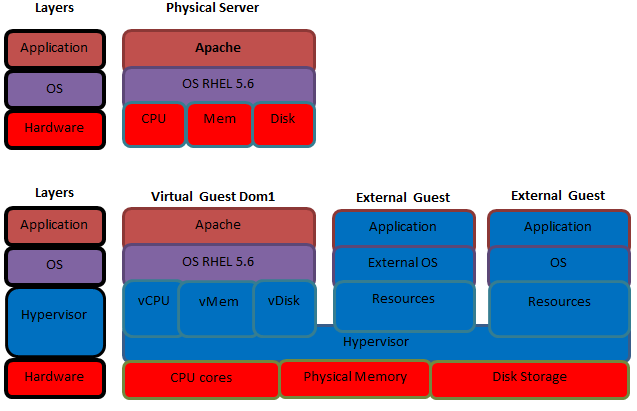
\includegraphics[width=6in]{images/LayersAndResources.png}
  \caption{New layer \textbf{Hypervisor} should share information with guest OS about physical resources.}
  \label{LayersAndResources}
  \end{center}
\end{figure}

The physical resource may be used by an external virtual machine or by the hypervisor, and there is little information that a guest OS or application can see about the physical resource.
Additional information is needed from hypervisor about the physical resource so that the administrator, OS, or application can make better decisions about the availability of the resource. 

\begin{table}[h]
  \begin{tabular}{ l p{10cm} }
    Resource & Definition \\
    \hline
    vCPU & The virtual core allocated to the guest \\
    vMemory & The virtual RAM allocated to the guest \\
    vDisk I/O & The virtual I/O block device allocated to the guest \\
    \hline
  \end{tabular}
\caption{Virtual resources which may experience interference from hypervisor or external guest.}
\label{tab:resources}
\end{table}

% 3 Identify the performance counters which can be used to measure I/O performance on a virtual guest machine.
\subsection{Performance statistics}
To monitor applications and the kernel, administration tools will read kernel statistics over some period of time.  Then the tool will aggregate and relate the data for that time period.  In some cases, additional inference can be made from different parts of the data.  For example the \emph{sar} utility can show the average wait time, average service time, and \emph{bandwidth utilization} for I/O.  On a physical server, where the hardware availability is relatively static, this information is valuable for analyzing and tuning applications.  However, when the resource is virtualized, these kernel resource statistics for virtual resources are almost meaningless.  Our tests will show that for disk I/O statistics, there is no difference between application changes and interference from external virtual guests. 

\begin{figure}[h]
\begin{algorithmic}[H]
 \STATE $interval \gets 5$
 \STATE $stat \gets$  DiskRead       
 \STATE $pre \gets $ READ $stat$ 
 \LOOP
    \STATE SLEEP $interval$
    \STATE $post \gets$ READ $stat$
    \STATE $result \gets (post - pre)/interval$
    \STATE PRINT  $result$
    \STATE $pre \gets post$ 
 \ENDLOOP
\end{algorithmic}
\caption{Example to display reads per second \emph{rd/s} every 5 seconds.}
\label{alg1}
\end{figure}

Our method will collect, aggregate, and analyze the statistics kept by the OS kernel in each guest domain and the hypervisor in order to measure interference from external domains and the hypervisor.  We find that there are kernel statistics that will show the interference from external machines, when collected from all layers.  For our examples we choose disk read and virtual memory statistics to analyze I/O bottlenecks.  However, this method could be used for identifying other types of performance problems if the data was available to the guest.

\begin{table}[h]
\begin{subtable}[h]{0.45\textwidth}
\caption{Virtual memory paging performance counters \cite{memory}}
\begin{tabular}{ l l }
       pgpgin  &  count of memory pages in. \\
       pgpgout  & count of memory pages out. \\
       pgfault  & count minor (or soft) page faults. \\
\end{tabular}
\label{fig:memory}
\end{subtable}
\hfill
\begin{subtable}[h]{0.45\textwidth}
\caption{I/O read performance counters \cite{iostats}}
\begin{tabular}{ l l }
       r\_sectors & number of sectors read successfully. \\
       r\_ms & number of milliseconds spent by all reads. \\
       r\_total & number of reads completed successfully. \\
\end{tabular}
\label{fig:io}
\end{subtable}
\caption{Statistics collected from all guests and hypervisor}
\end{table}

By collecting these statistics at two points in time as in algorithm \ref{alg1}, we can infer other data such as the throughput in reads per second \emph{r/s}.  However, the most import data we can infer is the disk I/O latency or the average wait time for reads \emph{AvgRdWait}.  
Since \emph{r\_ms} is the total number of milliseconds spent by all reads, we can divide this by the total number or read requests to get the average wait time.  This is very important since external guests may cause I/O delays in a shared disk.
\newline\newline
	$AvgRdWait = \frac{r\_ms}{r\_total}$ \\

% 4 A method to calculate the overhead and theoritical maximum performance using an offline modeling technique.
\subsection{Virtualization Overhead}
For each virtual resource (Table \ref{tab:resources}) there is a performance cost to making that resource virtualized.  If the guest had direct access to the hardware, at all times, the virtualization cost would be zero.  Since most system calls from the guest kernel need to go through the hypervisor, we need to account for this additional time.

Several researchers \cite{cherkasova, huber1} have called this cost the \emph{overhead}, and have quantified the overhead for a given configuration.  This previous research used an offline modeling technique by running a benchmark with and without virtualization.  By calculating the percent difference of these two benchmarks they can calculate the overhead.
The problem with this technique is that physical servers would need to be provisioned for this exercise.  Any configuration changes in hardware or anywhere in the software stack, may require a new test.  

Our method uses a similar approach, but does not require physcial harware for each guest.  We calculate the percent difference between the physical resources hypervisor and the virtual resources guest. 
We assert that the time spent waiting for an operation to complete in one layer depends on the layer below.  
In a physical server the application depends on the kernel and the kernel depends on the hardware.  
Our overhead calculation finds this additional time for I/O virtualization, by using the $AvgRdWait$ statistic in both the guest and hypervisor without interference to calculate the overhead.

We need to calculate the \emph{overhead} before running a guest virtual machine in production. 
In large scale datacenters and cloud systems, templates are usually created before virtual machines are used in production.  A template is a complete snapshot image of a virtual machine that has been built and tested to meet some need.  For example a Redhat 6.2 system with an Apache web server may need to be used on several machines.  A system could be built, tuned, and tested for that enviroment and then made into a template.  Future users can deploy a new virtual machine from that template.  We are suggesting to calculate the overhead from virtualization when it is made into a template.  

To calculate the virtualization overhead, create a single virtual machine with dedicated resources on isolated hardware.  
There are many performance benchmarks that can be used \cite{katcher, tikotekar, hplBench} to place a desired load on the virtual machine. 
Then place the load on the virtual machine and begin monitoring the performance statistics for that resource using the algorithm in Figure \ref{alg1} in BOTH the guest OS and hypervisor. 
Save the results of the guest, hypervisor, and time in the guest as this is the baseline statistic without external interference.
It is important that both the guest and hypervisor collect PRE and POST statistics as close to the same time as possible.  

Since we are measuring from the perspective of the guest OS, we want to discover how the guest degrades in comparison to the hypervisor.  
For some statistics such as the \emph{AvgRdWait}, we can approximate the overhead of virtualization, by calculating the average wait time in the hypervisor \emph{AvgRdWait\textsubscript{H}} and the guest \emph{AvgRdWait\textsubscript{G}}.

\begin{equation}
  Overhead_{IO} = \frac{AgvRdWait_G - AvgRdWait_H}{AvgRdWait_H} 
\end{equation}

\begin{figure}[h]
  \begin{center}
  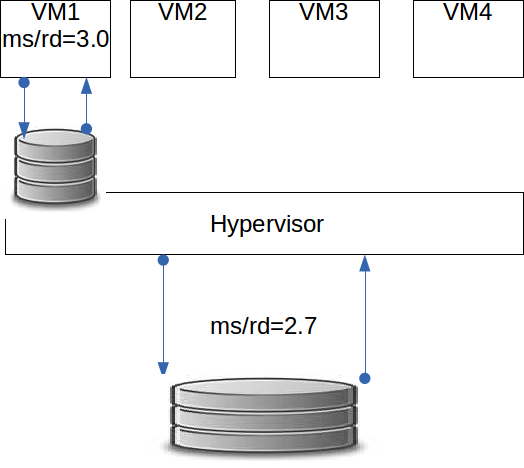
\includegraphics[width=3in]{images/RPS_single.png}
  \caption{The time waiting for I/O in the guest is greater than the I/O in the hypervisor. $Overhead_{IO}=10.2\%$}
  \label{RPSsingle}
  \end{center}
\end{figure}

% Simple method %
\subsection{Virtualization Interference}
The primary goal of the interference is to distinguish between a guest that is degraded because of an issue with the hypervisor layer (including external interference) and a guest that is degraded because of an application or OS layer issue.  In other words we should be able to distinguish between a problem in the guest and a problem which the guest has no control.  An secondary goal is to measure or analyze the interference.  We should be able to answer the question, "How much of the resource is available to the guest?".

A simple approach would simply show the interference from external machines by calculating the $AvgRdWait$ for the guest domain when calculating the overhead and when run with additional system and conclude that the interference is the difference between the two.  However, this would not (necessarily) describe the interference.  This would only show us that the resource is degraded for some reason.  In other words, by simply observing the time spent waiting in the guest or the quest I/O queue, we could not distinguish between a problem in the guest, hypervisor, or external system.

\subsection{External Interference}
When there is external interference the guest machine will be significantly degraded. 
When we also look at external layers (Figure \ref{int1}), we can see that other machines are sending data as well.  We can calculate the interference from external machines by calculating the sum of all the $ms/rd$ from all guest

\begin{equation}
  Overhead_V = \frac{count_G - count_H}{count_H} 
\end{equation}

% Picture with All guest numbers, "?" in hypervisor 
\begin{figure}[h]
  \begin{center}
  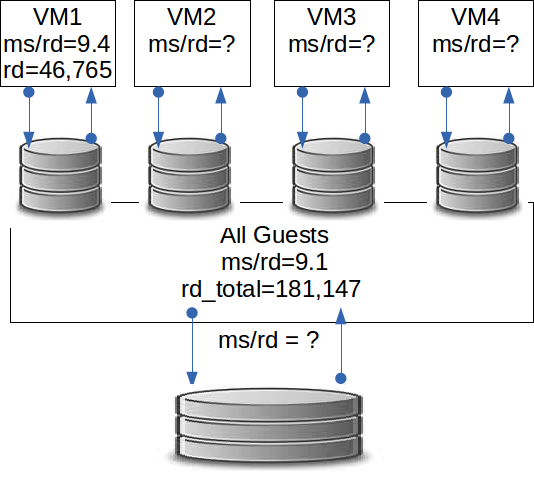
\includegraphics[width=3in]{images/RPS_int1.png}
  \caption{Guest 1 is degraded due to external interference.}
  \label{int1}
  \end{center}
\end{figure}

% A method to analyze performance of a guest machine which may be experiencing degredation from external interference.
\subsection{Hypervisor Interference}
It would not tell us if the resource was available to the guest.
We need to collect the same statistics from all guest systems, aggregate those counters, and compare that to the hypervisor.  We need to collect data from all of the layers of virtualization.

Since the guest has previously calculated $ Overhead_V $ we can use that information to calculate the interference when multiple guests are run concurrently $ Overhead_{Vall}$.  If all \emph{n} guests have been modified to collect and pass information to the hypervisor, each guest can reply with their counters when asked by the hypervisor.  It is important that all guests and the hypervisor start and stop counting concurrently to provide accurate results.  

\begin{equation}
Overhead_{Vall} = \frac{count_{Gall} - count_H}{count_{Gall}} 
\label{eq2}
\end{equation}

\indent We can see that when the number of guests machines is 1 (as when we collected the overhead with 1 machine), this is exactly as equation 1.  After the hypervisor calculates the count and overhead for all machines running and passes this information to the original guest, the guest can then calculate the interference.  
The interference from other virtual machines $Interference_V$ is calculated by subtracting the overhead from all guests from the original overhead found without any external interference. 

\begin{equation}
Interference_V = Overhead_{Vall} - Overhead_V
\label{eq3}
\end{equation}


\begin{equation}
	Count_{Gall} = \sum_{i=1}^n{count_G} 
\end{equation}

% TODO Algoritm 
\begin{enumerate}
	\item Guest tool requests OS permance counter statistics.
	\item Guest OS forwards request to hypervisor.
	\item Hypervisor forwards request to all guests.
	\item Hypervisor begins monitoring for specified time and waits determined time.
	\item Each Guest responds with individual statistics.
	\item Hypervisor calculates $Overhead_{Vall}$ (Equation 2) of resource used.
	\item Hypervisor returns $Overhead_{Vall}$ to original requestor.
	\item Guest calculates the $Interference$ (Equation 3).
\end{enumerate}

\indent As an example: the userspace tool \emph{iostat} reads disk performance counters in /proc/diskstats and will report transfers, bytes read, and bytes written per second.  If an application was experiencing I/O performance problems this would be a tool an administrator or application developer may monitor.  Without knowing the interference this could be misleading as to the root cause of the problem.  The following example shows a possible output from the perspective of the running guest when experiencing I/O interference from external guest machines.

\begin{figure}[h]
\begin{Verbatim}
Device:  tps    kB_read/s    kB_wrtn/s
sda   577.20     41388.00    148073.00
 virtual I/O interference 22.4%     
\end{Verbatim}
\label{fig:iostat}
\caption{Example:  \emph{iostat} with additional calculated interference.}
\end{figure}

